\chapter{System Architecture}
\label{chap:arch}

This chapter presents information concerning the architecture of the software
system both from the static and dynamic viewpoints. The static viewpoint focuses
on the physical architecture (hardware) required to deploy and run the
software system along with the manner in which the components that make such
software system are grouped. On the other hand, the dynamic viewpoint focuses on
the behaviour of the software system at runtime. 

The static information is presented through the \gls{Deployment View} and the
\gls{Implementation View}. The dynamic aspects of the system are presented by
means of the \gls{UI Processing View}.


\section{Deployment view}
The aim of the \gls{Deployment View} is to describe the different processing nodes that compose
the deployment infrastructure and how they are interconnected. A processing node
corresponds to a piece of hardware aimed at executing either the whole software
system or a sub-part of it.

\begin{figure}[h]
	\centering
	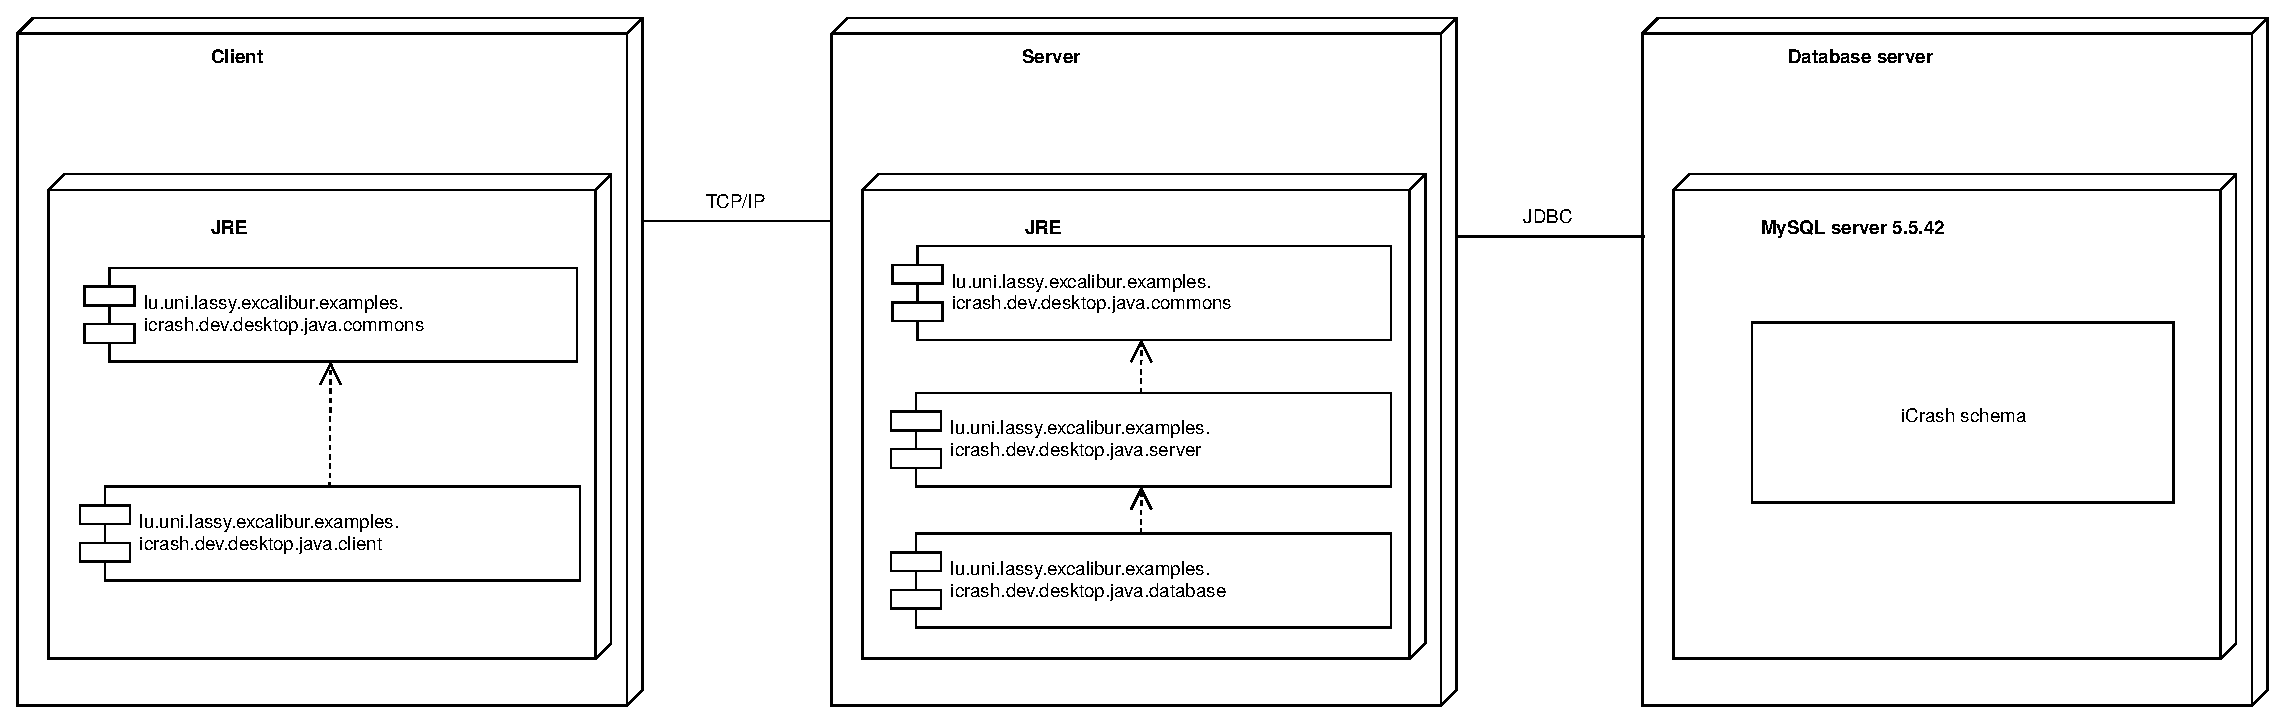
\includegraphics[width=0.9\textwidth]{./images/architecture/deployment_view.eps}
	\caption{Deployment View Diagram}
\end{figure}


\section{Implementation view}
The \gls{Implementation View} describes each software system component and how
they are organised and combined to make the targeted software system.

\begin{figure}[h!]
	\centering
	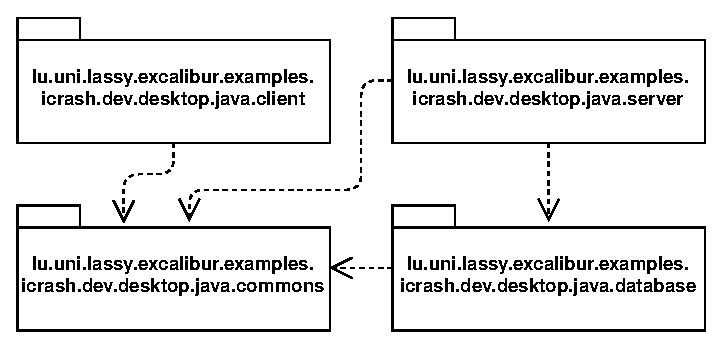
\includegraphics[width=0.9\textwidth]{./images/architecture/implementation_view/highest_view.eps}
	\caption{Implementation View - High level}
\end{figure}

\subsection{Common Component}
\begin{figure}[h!]
	\centering
	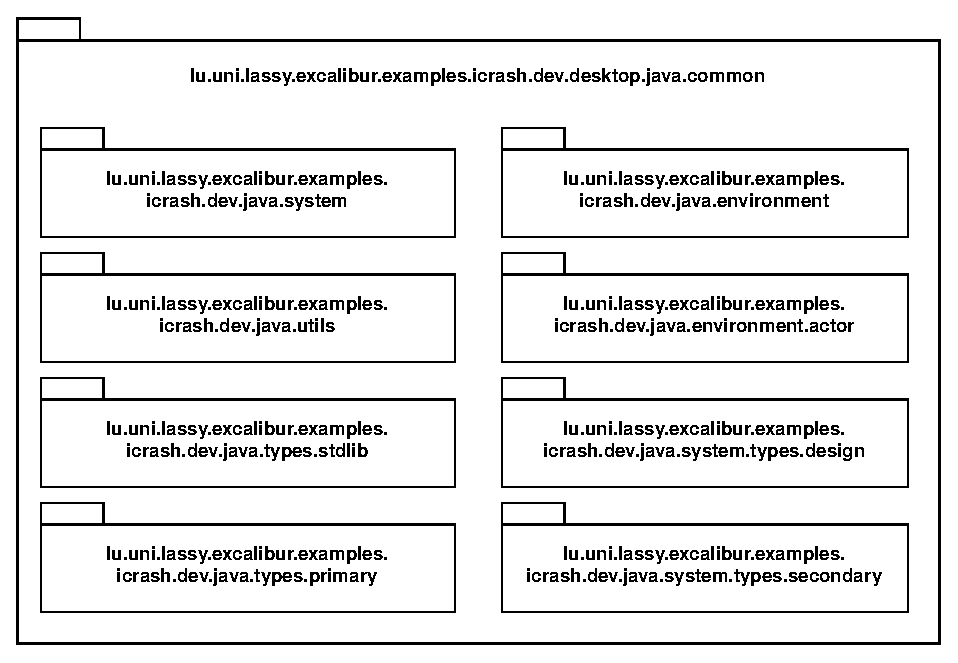
\includegraphics[width=0.9\textwidth]{./images/architecture/implementation_view/commons_project.eps}
	\caption{Implementation View - Common Component}
\end{figure}

\subsection{Component Database project}
\begin{figure}[h!]
	\centering
	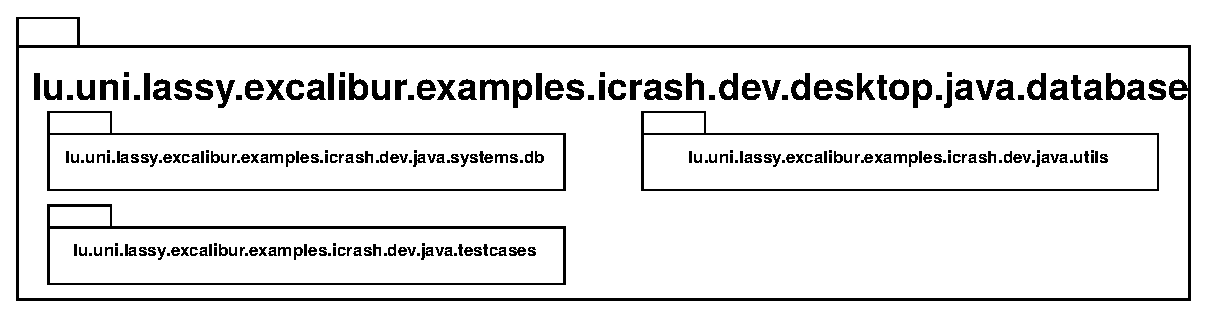
\includegraphics[width=0.9\textwidth]{./images/architecture/implementation_view/database_project.eps}
	\caption{Implementation View - Common Component}
\end{figure}

\subsection{Component Server project}
\begin{figure}[h!]
	\centering
	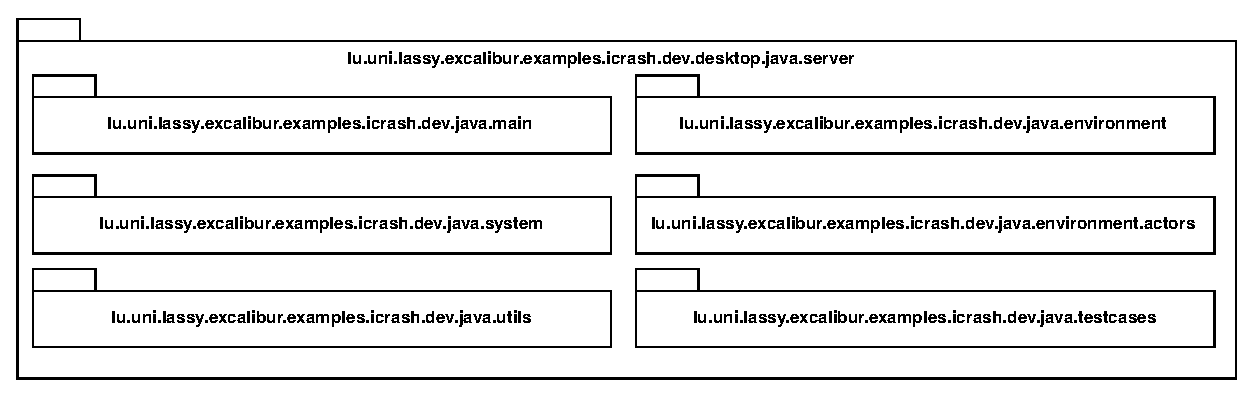
\includegraphics[width=0.9\textwidth]{./images/architecture/implementation_view/server_project.eps}
	\caption{Implementation View - Common Component}
\end{figure}


\subsection{Component Client project}
\begin{figure}[h!]
	\centering
	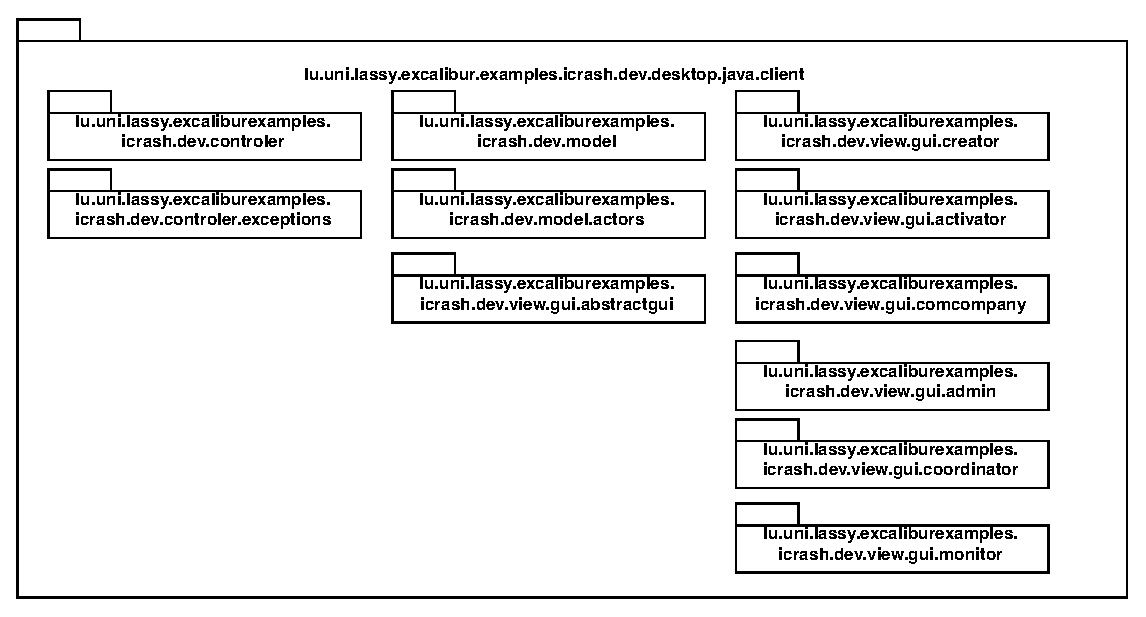
\includegraphics[width=0.9\textwidth]{./images/architecture/implementation_view/client_project.eps}
	\caption{Implementation View - Common Component}
\end{figure}



\section{UI Processing view}
A \gls{UI Processing View} is aimed at explaining the required message exchanges
to achieve the launching of a system operation (specified in the \msrmessir
Analysis Document). These required message exchanges (which are not specified in
the \msrmessir Analysis Document) make part of the user interface (UI). Thus, the
main interest of a UI Processing View is to describe the design choices made
at the UI level, such that a system operation is launched. The description
of a UI Processing View is given by means of a UML Sequence Diagram. 


%A complete Design Document should contain a UI Processing View for each
%non-proactive system operation specified in the \msrmessir Analysis Document,
% as such kind of system operations are launched by actors through UIs that allows
%them to make so. 

\subsection{UI Processing view for system operation oeSetClock}
\begin{figure}[h!]
	\centering
	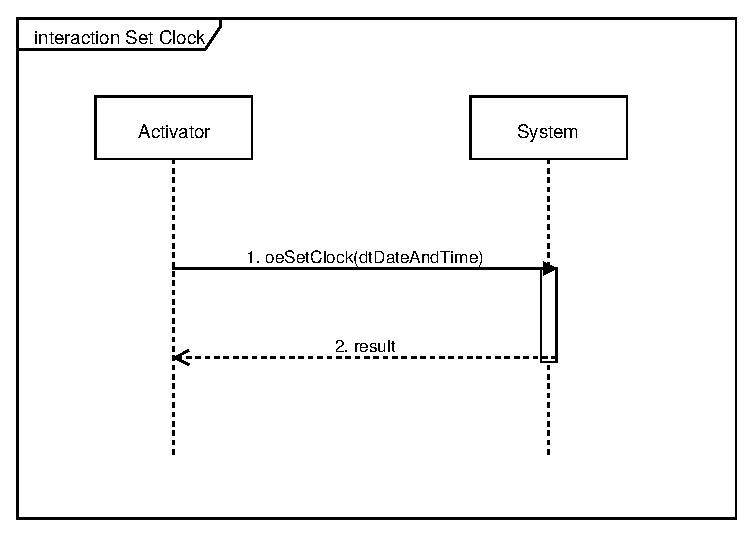
\includegraphics[width=0.9\textwidth]{./images/architecture/processing_view/set_clock.eps}
	\caption{Processing View - Set Clock}
\end{figure}


\subsection{UI Processing view for system operation oeSystemOperation1}
TODO

 
\subsection{UI Processing view for system operation oeSystemOperation2}
TODO


\subsection{UI Processing view for system operation oeSystemOperation3}
TODO





\section{Non-functional runtime concerns}
The description of the runtime processes in terms of concurrency, distribution,
performance and scalability aspects.

\subsection{Performance}
System uses all the performance capabilities provided by hosted Java Virtual
Machine and MySQL dabase.

\subsection{Concurrency and Parallelism}
The concurrency and parallelism is provided by Java and MySQL in the GUI and
actor request handling.

\subsection{Scalability}
Horizontal scalability is possible only for database system which is provided
by means of MySQL. As for other parts, scalability can be achieved in vertical
manner for client and server parts of the system. 
